%package list
\documentclass{article}
\usepackage[top=3cm, bottom=3cm, outer=3cm, inner=3cm]{geometry}
\usepackage{multicol}
\usepackage{graphicx}
\usepackage{url}
%\usepackage{cite}
\usepackage{hyperref}
\usepackage{array}
%\usepackage{multicol}
\newcolumntype{x}[1]{>{\centering\arraybackslash\hspace{0pt}}p{#1}}
\usepackage{natbib}
\usepackage{pdfpages}
\usepackage{multirow}
\usepackage[normalem]{ulem}
\useunder{\uline}{\ul}{}
\usepackage{svg}
\usepackage{xcolor}
\usepackage{listings}
\lstdefinestyle{ascii-tree}{
	literate={├}{|}1 {─}{--}1 {└}{+}1 
}
\lstset{basicstyle=\ttfamily,
	showstringspaces=false,
	commentstyle=\color{red},
	keywordstyle=\color{blue}
}
%\usepackage{booktabs}
\usepackage{caption}
\usepackage{subcaption}
\usepackage{float}
\usepackage{array}

\newcolumntype{M}[1]{>{\centering\arraybackslash}m{#1}}
\newcolumntype{N}{@{}m{0pt}@{}}


%%%%%%%%%%%%%%%%%%%%%%%%%%%%%%%%%%%%%%%%%%%%%%%%%%%%%%%%%%%%%%%%%%%%%%%%%%%%
%%%%%%%%%%%%%%%%%%%%%%%%%%%%%%%%%%%%%%%%%%%%%%%%%%%%%%%%%%%%%%%%%%%%%%%%%%%%
\newcommand{\itemEmail}{jchuraaca@unsa.edu.pe}
\newcommand{\itemStudent}{Julio Rubén Chura Acabana}
\newcommand{\itemCourse}{ F. de Programción 2}
\newcommand{\itemCourseCode}{20230472}
\newcommand{\itemSemester}{I}
\newcommand{\itemUniversity}{Universidad Nacional de San Agustín de Arequipa}
\newcommand{\itemFaculty}{Facultad de Ingeniería de Producción y Servicios}
\newcommand{\itemDepartment}{Departamento Académico de Ingeniería de Sistemas e Informática}
\newcommand{\itemSchool}{Escuela Profesional de Ingeniería de Sistemas}
\newcommand{\itemAcademic}{2023 - B}
\newcommand{\itemInput}{Del 8 de Enero 2023}
\newcommand{\itemOutput}{Al 10 de Enero 2023}
\newcommand{\itemPracticeNumber}{20}
\newcommand{\itemTheme}{Clase Ejército – Soldado – Mapa. Herencia y Polimorfismo. Miembros de clase}
%%%%%%%%%%%%%%%%%%%%%%%%%%%%%%%%%%%%%%%%%%%%%%%%%%%%%%%%%%%%%%%%%%%%%%%%%%%%
%%%%%%%%%%%%%%%%%%%%%%%%%%%%%%%%%%%%%%%%%%%%%%%%%%%%%%%%%%%%%%%%%%%%%%%%%%%%

\usepackage[english,spanish]{babel}
\usepackage[utf8]{inputenc}
\AtBeginDocument{\selectlanguage{spanish}}
\renewcommand{\figurename}{Figura}
\renewcommand{\refname}{Referencias}
\renewcommand{\tablename}{Tabla} %esto no funciona cuando se usa babel
\AtBeginDocument{%
	\renewcommand\tablename{Tabla}
}

\usepackage{fancyhdr}
\pagestyle{fancy}
\fancyhf{}
\setlength{\headheight}{30pt}
\renewcommand{\headrulewidth}{1pt}
\renewcommand{\footrulewidth}{1pt}
\fancyhead[L]{\raisebox{-0.2\height}{
\includegraphics[width=3cm]{img/logo_episunsa.png}}}
\fancyhead[C]{\fontsize{7}{7}\selectfont	\itemUniversity \\ \itemFaculty \\ \itemDepartment \\ \itemSchool \\ \textbf{\itemCourse}}
\fancyhead[R]{\raisebox{-0.2\height}{
\includegraphics[width=1.2cm]{img/logo_abet}}}
\fancyfoot[L]{Estudiante Julio Rubén Chura Acabana}
\fancyfoot[C]{\itemCourse}
\fancyfoot[R]{Página \thepage}

% para el codigo fuente
\usepackage{listings}
\usepackage{color, colortbl}
\definecolor{dkgreen}{rgb}{0,0.6,0}
\definecolor{gray}{rgb}{0.5,0.5,0.5}
\definecolor{mauve}{rgb}{0.58,0,0.82}
\definecolor{codebackground}{rgb}{0.95, 0.95, 0.92}
\definecolor{tablebackground}{rgb}{0.8, 0, 0}

\lstset{frame=tb,
	language=bash,
	aboveskip=3mm,
	belowskip=3mm,
	showstringspaces=false,
	columns=flexible,
	basicstyle={\small\ttfamily},
	numbers=none,
	numberstyle=\tiny\color{gray},
	keywordstyle=\color{blue},
	commentstyle=\color{dkgreen},
	stringstyle=\color{mauve},
	breaklines=true,
	breakatwhitespace=true,
	tabsize=3,
	backgroundcolor= \color{codebackground},
}

\begin{document}
	
	\vspace*{10px}
	
	\begin{center}	
		\fontsize{17}{17} \textbf{ Informe de Laboratorio \itemPracticeNumber}
	\end{center}
	\centerline{\textbf{\Large Tema: \itemTheme}}
	%\vspace*{0.5cm}	
	
	\begin{flushright}
		\begin{tabular}{|M{2.5cm}|N|}
			\hline 
			\rowcolor{tablebackground}
			\color{white} \textbf{Nota}  \\
			\hline 
			\\[30pt]
			\hline 			
		\end{tabular}
	\end{flushright}	
	
	\begin{table}[H]
		\begin{tabular}{|x{4.7cm}|x{4.8cm}|x{4.8cm}|}
			\hline 
			\rowcolor{tablebackground}
			\color{white} \textbf{Estudiante} & \color{white}\textbf{Escuela}  & \color{white}\textbf{Asignatura}   \\
			\hline 
			{\itemStudent \par \itemEmail} & \itemSchool & {\itemCourse \par Semestre: \itemSemester \par Código: \itemCourseCode}     \\
			\hline 			
		\end{tabular}
	\end{table}		
	
	\begin{table}[H]
		\begin{tabular}{|x{4.7cm}|x{4.8cm}|x{4.8cm}|}
			\hline 
			\rowcolor{tablebackground}
			\color{white}\textbf{Laboratorio} & \color{white}\textbf{Tema}  & \color{white}\textbf{Duración}   \\
			\hline 
			\itemPracticeNumber & \itemTheme & 04 horas   \\
			\hline 
		\end{tabular}
	\end{table}
	
	\begin{table}[H]
		\begin{tabular}{|x{4.7cm}|x{4.8cm}|x{4.8cm}|}
			\hline 
			\rowcolor{tablebackground}
			\color{white}\textbf{Semestre académico} & \color{white}\textbf{Fecha de inicio}  & \color{white}\textbf{Fecha de entrega}   \\
			\hline 
			\itemAcademic & \itemInput &  \itemOutput  \\
			\hline 
		\end{tabular}
	\end{table}
	
	\section{Tarea}
	\begin{itemize}		
		\item En este laboratorio deberá hacer uso de los conceptos de Herencia, Polimorfismo y composición.Para ello deberá crear diversas clases y culminada la actividad, deberá elaborar un informe 
	\end{itemize}
	
	\section{Equipos, materiales y temas utilizados}
	\begin{itemize}
		\item Sistema Operativo Windows
		\item Visual Studio Code 1.85.1
		\item OpenJDK 64-Bits 20.0.2.
		\item Git 2.42.0.
		\item Cuenta en GitHub con el correo institucional.
		\item Herencia y Polimorfismo
	\end{itemize}
	
	\section{URL de Repositorio Github}
	\begin{itemize}
		\item URL del Repositorio GitHub para clonar o recuperar.
		\item \url{https://github.com/JulioChura/fp2-23b.git}
		\item URL para el laboratorio 01 en el Repositorio GitHub.
		\item \url{https://github.com/JulioChura/fp2-23b/tree/main/fase02/lab20}
	\end{itemize}
	
	\section{Actividades con el repositorio GitHub}
	
	
	
	
	
	
	
	\subsection{Preparación del espacio de trabajo}
	
	\begin{lstlisting}[language=bash,caption={Se crea la carpeta de laboratorio 20 y se copian los archivos del lab012 al lab20 }][H]
		mkdir lab20
		cd lab20
		Copy-Item "Soldier.java" -Destination "..\lab20"
		Copy-Item "VideoJuego5.java" -Destination "..\lab12\VideoJuego.java"
		cd ..
		cd lab20
		code .
	\end{lstlisting}
	
	\begin{lstlisting}[language=bash,caption={Commit: 99f16a3c517c18d8206b100d33722e5805398f60 }][H]
		git add Soldier.java
		git commit -m "Se copia las clase Soldier.java y VideoJuego.java del lab12 al 20"
		git push -u origin main
	\end{lstlisting}
	

	
	\subsection{Aplicación de la Herencia}
	\begin{lstlisting}[language=bash,caption={Se modifican metodos de la clase Soldier }][H]
		code Soldier.java
	\end{lstlisting}
	\begin{figure}[H]
		\centering
		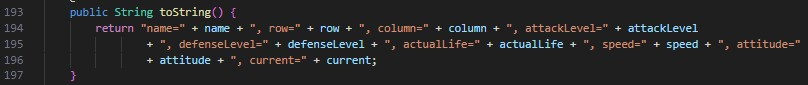
\includegraphics[width=1\textwidth,keepaspectratio]{img/toString.jpg}
		%\includesvg{img/automata.svg}
		%\label{img:mot2}
		%\caption{Product backlog.}
	\end{figure}
	
	\begin{itemize}	
		\item Como las demás clases heredarán de Soldier sus métodos y atributos, para una mejor visualización de los datos de la clase, se corrige la forma en la que el toString de la versión anterior mostraba   
	\end{itemize}
	
	
	
	
	\begin{lstlisting}[language=bash,caption={Se crea la subclase Archer }][H]
		code Archer.java
	\end{lstlisting}
	\begin{figure}[H]
		\centering
		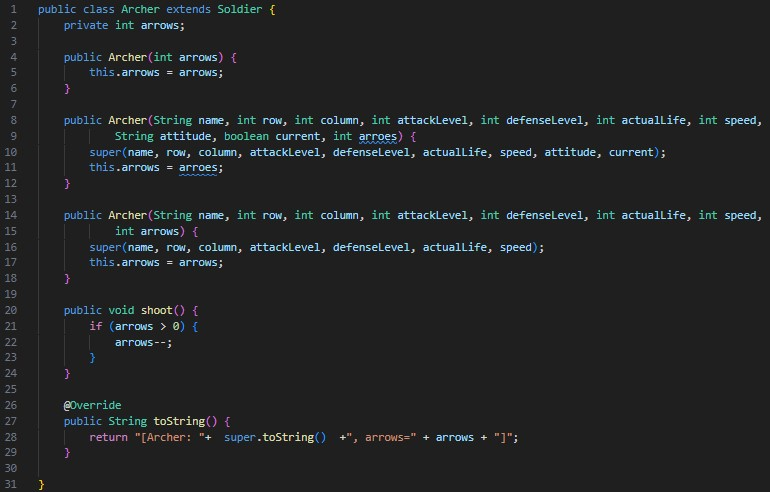
\includegraphics[width=1\textwidth,keepaspectratio]{img/archer.jpg}
		%\includesvg{img/automata.svg}
		%\label{img:mot2}
		%\caption{Product backlog.}
	\end{figure}	
	\begin{lstlisting}[language=bash,caption={Commit: c3fab4bac8b4e5e7a1463ecc8e1f205b3f755977 }][H]
		git add Archer.java
		git commit -m "Se crea el metodo shoot y el toString"			
		git push -u origin main
	\end{lstlisting}
	
	
	

	\begin{lstlisting}[language=bash,caption={Se crea la subclase Knight }][H]
		code Knight.java
	\end{lstlisting}
	\begin{figure}[H]
		\centering
		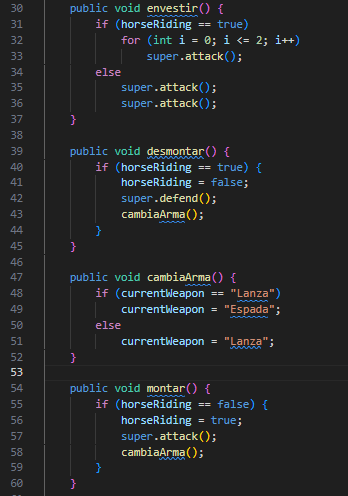
\includegraphics[width=1\textwidth,keepaspectratio]{img/knight.png}
		%\includesvg{img/automata.svg}
		%\label{img:mot2}
		%\caption{Product backlog.}
	\end{figure}
	\begin{itemize}	
		\item Este fragmento es lo más interesante de esta clase y lo que la práctica de laboratorio específica  
	\end{itemize}	
	\begin{lstlisting}[language=bash,caption={Commit: a4b277fea2814d4543b4b906fc545da59c009198 }][H]
		git add Knight.java
		git commit -m "Se agrega la funcion attack dentro de envestir"			
		git push -u origin main
	\end{lstlisting}
	
	
	\begin{lstlisting}[language=bash,caption={Se crea la subclase Spearman }][H]
		code Spearman.java
	\end{lstlisting}
	\begin{figure}[H]
		\centering
		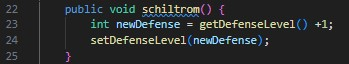
\includegraphics[width=1\textwidth,keepaspectratio]{img/spearman.jpg}
		%\includesvg{img/automata.svg}
		%\label{img:mot2}
		%\caption{Product backlog.}
	\end{figure}
	\begin{itemize}	
		\item Este fragmento es lo más interesante de esta clase y lo que la práctica de laboratorio específica  
	\end{itemize}	
	\begin{lstlisting}[language=bash,caption={Commit: 2039a89dc9095c3a2a7acd26f64f5efeddae5e23 }][H]
		git add Spearman.java
		git commit -m "Se implementa el metodo schiltrom"			
		git push -u origin main
	\end{lstlisting}
	
	

	\begin{lstlisting}[language=bash,caption={Se crea la subclase Swordsman }][H]
		code Swordsman.java
	\end{lstlisting}
	\begin{figure}[H]
		\centering
		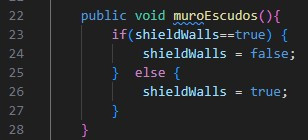
\includegraphics[width=1\textwidth,keepaspectratio]{img/muro.jpg}
		%\includesvg{img/automata.svg}
		%\label{img:mot2}
		%\caption{Product backlog.}
	\end{figure}
	\begin{itemize}	
		\item Este fragmento es lo más interesante de esta clase y lo que la práctica de laboratorio específica  
	\end{itemize}	
	\begin{lstlisting}[language=bash,caption={Commit: 82b0ba62ff23779dc047659700c9991032678c3b }][H]
		git add Swordsman.java
		git commit -m "Se crea el metodo muroEscudos y el toString se sobreescribe"			
		git push -u origin main
	\end{lstlisting}
	
	
	\subsection{Aplicación de Composición}
	
	\begin{lstlisting}[language=bash,caption={Se crea la Army}][H]
		code Army.java
	\end{lstlisting}
	\begin{figure}[H]
		\centering
		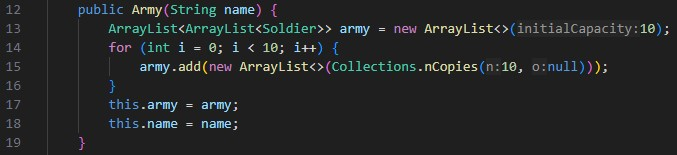
\includegraphics[width=1\textwidth,keepaspectratio]{img/constructorArmy.jpg}
		%\includesvg{img/automata.svg}
		%\label{img:mot2}
		%\caption{Product backlog.}
	\end{figure}
	\begin{itemize}	
		\item Este fragmento ya establece a los atributos ArrayList valores null y establece el nombre de cada ejercito que se creé  
	\end{itemize}	
	\begin{lstlisting}[language=bash,caption={Commit: 2f415f95bd8470ae0b16e5a2c7af7d2fdfb1a841 }][H]
		git add Army.java
		git commit -m "Se crean 3 constructores sobrecargados"			
		git push -u origin main
	\end{lstlisting}
	
	
	
	

	\begin{lstlisting}[language=bash,caption={Se crea generateArmy}][H]
		code Army.java
	\end{lstlisting}
	\begin{figure}[H]
		\centering
		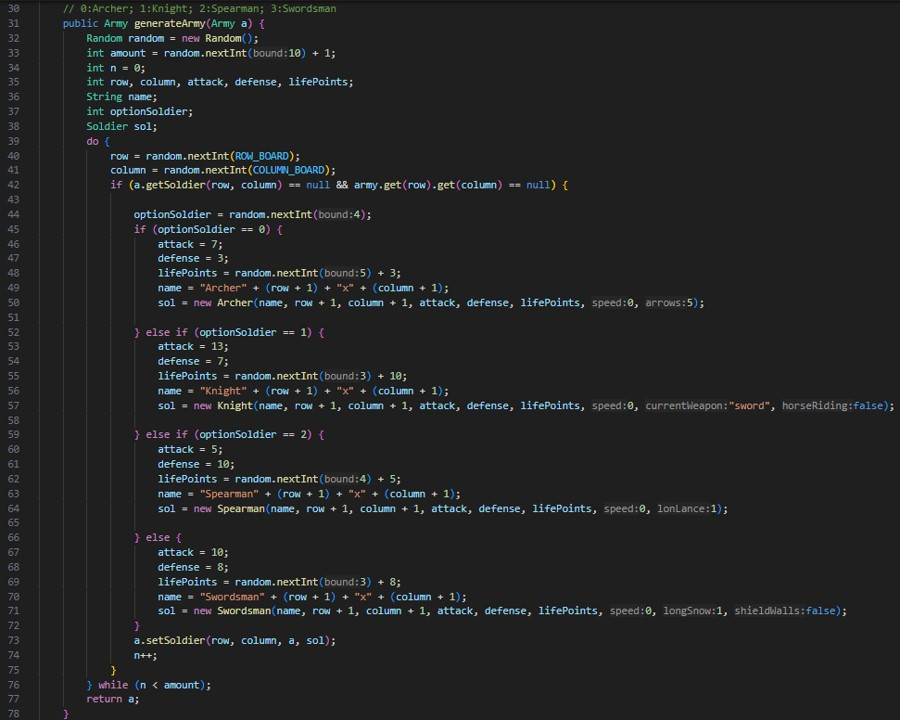
\includegraphics[width=1\textwidth,keepaspectratio]{img/generateArmy.jpg}
		%\includesvg{img/automata.svg}
		%\label{img:mot2}
		%\caption{Product backlog.}
	\end{figure}
	\begin{itemize}	
		\item Este método guarda la misma lógica para generar el ejército del lab12, solo que aquí se nos pide incluir dentro del ejército soldados que son de la clase hija, por lo que se hace uso del Polimorfismo. Para agregar los soldados de las clases hija se hace de forma aleatoria 
	\end{itemize}	
	\begin{lstlisting}[language=bash,caption={Commit: cd5e2d1a4c71b2db3ae28978a840f7c4ff318738 }][H]
		git add Army.java
		git commit -m "Se termina de generar soldados de todos los tipos por ejercito"			
		git push -u origin main
	\end{lstlisting}
	
	
	
	
	
	
	\begin{lstlisting}[language=bash,caption={Se crean métodos que nos permitirán acceder a los atributos de ña clase}][H]
		code Army.java
	\end{lstlisting}
	\begin{figure}[H]
		\centering
		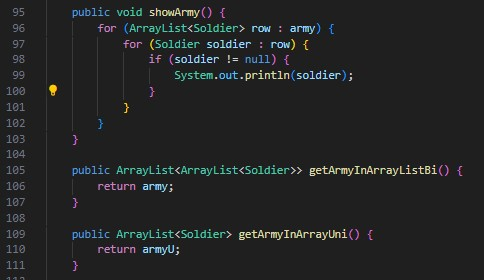
\includegraphics[width=1\textwidth,keepaspectratio]{img/getArmy.jpg}
		%\includesvg{img/automata.svg}
		%\label{img:mot2}
		%\caption{Product backlog.}
	\end{figure}
	\begin{itemize}	
		\item Estos métodos nos permiten visualizar los soldier de cada ejército y obtener los atributos que son ArrayList. Antes de estos métodos venía otro el cual convertía ArrrayList Bidimensionales en Unidimensionales, prácticamente se copió este método de la clase VideoJuego a la clase Army  
	\end{itemize}	
	\begin{lstlisting}[language=bash,caption={Commit: 0f87b3ab9106b3b59a30c056e21495671d0e5fa2 }][H]
		git add Army.java
		git commit -m "Se crean metodos que nos serviran para acceder al atributo que es de
	tipo ArraList de la clase Army y tambien podremos visualizar los soldier de cada ejercito"			
		git push -u origin main
	\end{lstlisting}
	
	
	
	\begin{lstlisting}[language=bash,caption={Se termina de crear los demás métodos}][H]
		code Army.java
	\end{lstlisting}
	\begin{figure}[H]
		\centering
		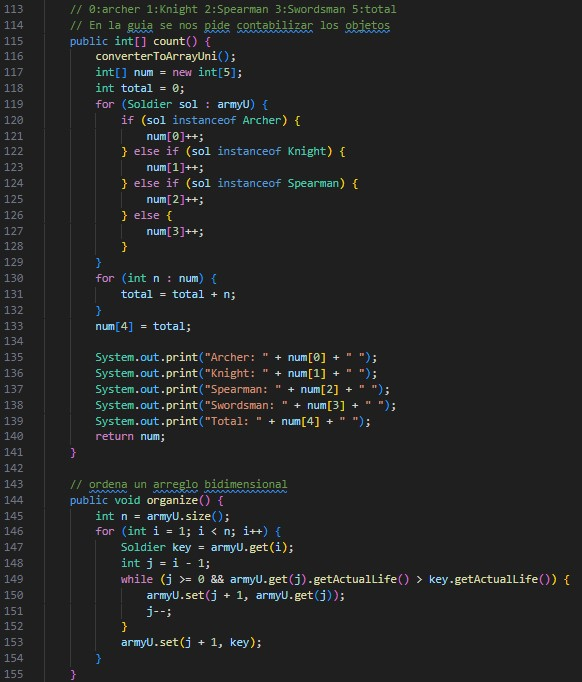
\includegraphics[width=1\textwidth,keepaspectratio]{img/otherArmy.jpg}
		%\includesvg{img/automata.svg}
		%\label{img:mot2}
		%\caption{Product backlog.}
	\end{figure}
	\begin{itemize}	
		\item Se crearon otros métodos pero en su mayoría solo son accesores y que básicamente necesitan de estos dos para poder funcionar. Count nos devuelve la cantidad de soldados y también hace la contabilización de las subclases hijas. En cuanto al método Organize usa un método de ordenamiento, este método ya se vino trabajando en laboratorios pasados, solo que en esta versión se le adapta para que sea un método de clase y no estático como lo era antes  
	\end{itemize}	
	\begin{lstlisting}[language=bash,caption={Commit: 0f87b3ab9106b3b59a30c056e21495671d0e5fa2 }][H]
		git add Board.java
		git commit -m "Se crean metodos que nos serviran para acceder al atributo que es de
		tipo ArraList de la clase Army y tambien podremos visualizar los soldier de cada ejercito"			
		git push -u origin main
	\end{lstlisting}
	
	
	

	\subsection{Clase Board}
	
	\begin{lstlisting}[language=bash,caption={Se crean los métodos que generan caracteres para el tablero}][H]
		code Board.java
	\end{lstlisting}
	\begin{figure}[H]
		\centering
		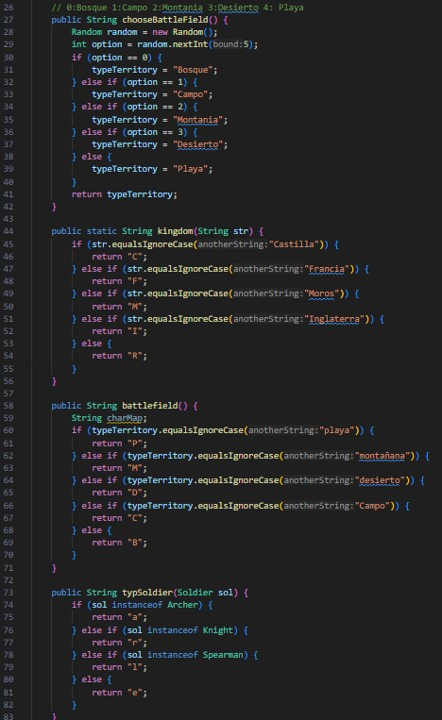
\includegraphics[width=0.8\textwidth,keepaspectratio]{img/chars.jpg}
		%\includesvg{img/automata.svg}
		%\label{img:mot2}
		%\caption{Product backlog.}
	\end{figure}
	\begin{itemize}	
		\item Por supuesto que antes de crear estos métodos ya se han creado los atributos y el constructor. El constructor recibe como parámetros dos objetos de clase Army  (se evidencia aquí más el uso de la composición). En cuanto a los métodos de la presente imagen, se limitan a poder establecer los carácteres que se imprimirán en el tablero
	\end{itemize}	
	\begin{lstlisting}[language=bash,caption={Commit: 4c61c72b558e8335ed0dda950c796c2caaa121e0 }][H]
		git add Board.java
		git commit -m "Se crean metodos que generan un caracter para el tablero"			
		git push -u origin main
	\end{lstlisting}
	
	
	\begin{lstlisting}[language=bash,caption={Se modifica la impresión del tablero}][H]
		code Board.java
	\end{lstlisting}
	\begin{figure}[H]
		\centering
		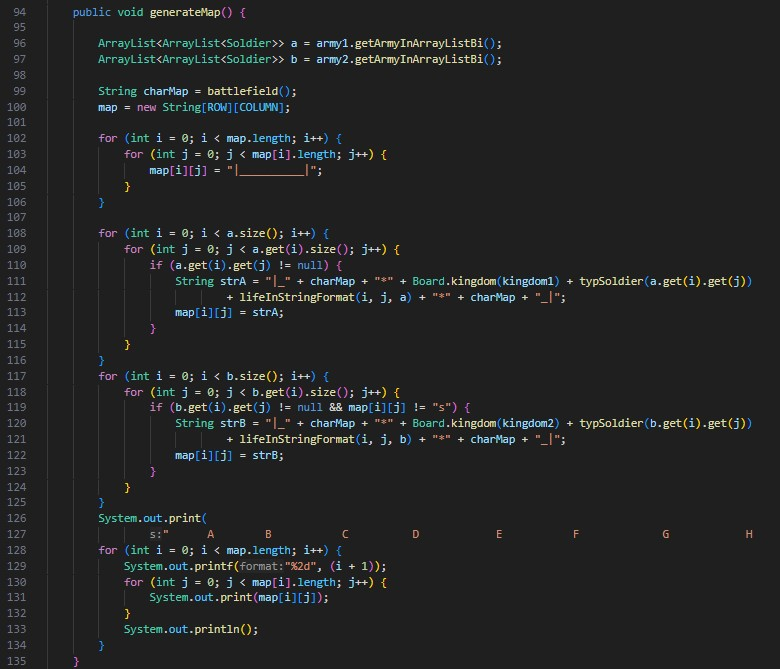
\includegraphics[width=1\textwidth,keepaspectratio]{img/printBoard.jpg}
		%\includesvg{img/automata.svg}
		%\label{img:mot2}
		%\caption{Product backlog.}
	\end{figure}
	\begin{itemize}	
		\item La lógica con la que se genera el tablero no ha cambiado, solo se hacen leves modificaciones como la inclusión de nuevos caracteres que simulan el tipo de arena, el reino, el tipo o clase de soldado que es, su valor de vida actual y por ultimo se vuelve a poner el carácter que simula el ambiente del combate 
	\end{itemize}	
	\begin{lstlisting}[language=bash,caption={Commit: ea7d152254cd6643d1efa6457507b9b3f09e5c5f }][H]
		git add Board.java
		git commit -m "Se modifica el metodo myBoard que era estatico, ahora es un metodo de clase y tambien se le cambio el nombre al metodo"			
		git push -u origin main
	\end{lstlisting}

	
	
	\subsection{Clase GameFast}
		
	\begin{lstlisting}[language=bash,caption={Se crea la clase que gestiona el juego}][H]
		code GameFast.java
	\end{lstlisting}
	\begin{figure}[H]
		\centering
		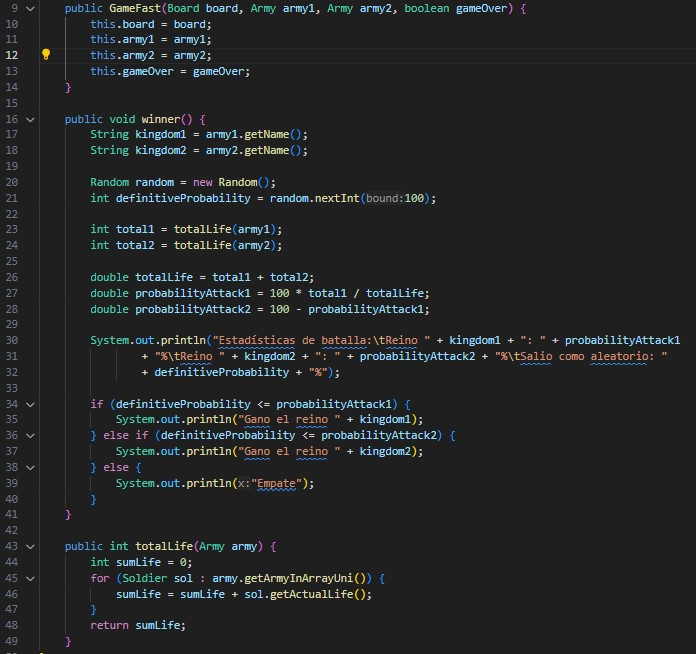
\includegraphics[width=1\textwidth,keepaspectratio]{img/gameFast.jpg}
		%\includesvg{img/automata.svg}
		%\label{img:mot2}
		%\caption{Product backlog.}
	\end{figure}
	\begin{itemize}	
		\item En esta imagen solo se verá dos métodos que son importantes, el primero es winner que cual dictamina al ganador mediante el criterio de probabilidades, por ejemplo si un ejército sacó 30 por ciento, mientras que el otro 70 y la probabilidad definitiva es es 23 por ciento, el primer ejército gana ya que está dentro de su rango. Sin embargo, para que este método pueda hacer su función requiere la suma total de los puntos de vida de cada army, por lo que se crea el método totalLife el cual calcula ello. 
	\end{itemize}	
	\begin{lstlisting}[language=bash,caption={Commit: 289acd859314fecd76473faa1f7adbae3f3de7c0 }][H]
		git add GameFast.java
		git commit -m "Se crean los metodos winner y totalLife de GameFast"			
		git push -u origin main
	\end{lstlisting}
	
	
	
	\subsection{Clase Aplicación y ejecución del programa}
	
	
	\begin{lstlisting}[language=bash,caption={Se crea la clase principal que llama a todas las clases}][H]
		code Aplicacion.java
	\end{lstlisting}
	\begin{figure}[H]
		\centering
		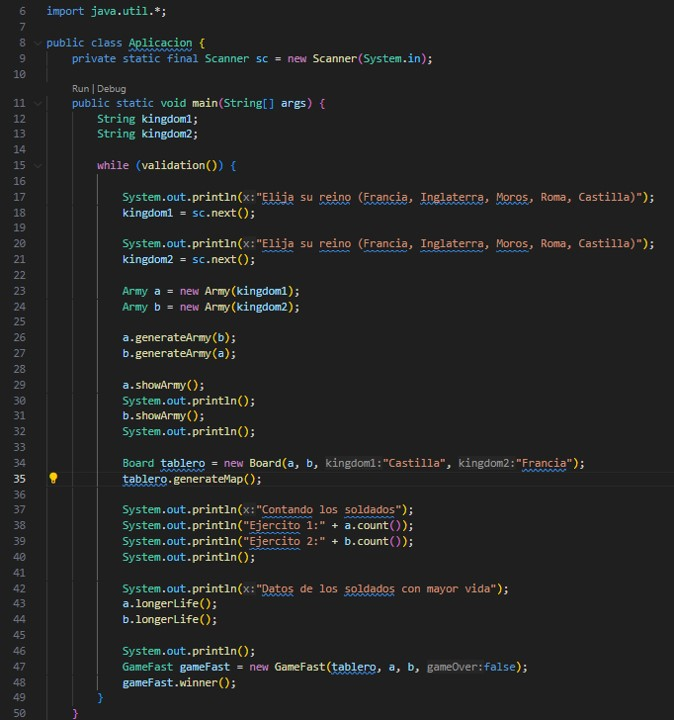
\includegraphics[width=1\textwidth,keepaspectratio]{img/main.jpg}
		%\includesvg{img/automata.svg}
		%\label{img:mot2}
		%\caption{Product backlog.}
	\end{figure}
	\begin{itemize}	
		\item Básicamente esta clase es la principal ya que se encarga de la ejecución de todo el programa. Se hace un juego iterativo.
	\end{itemize}
	
	\begin{figure}[H]
		\centering
		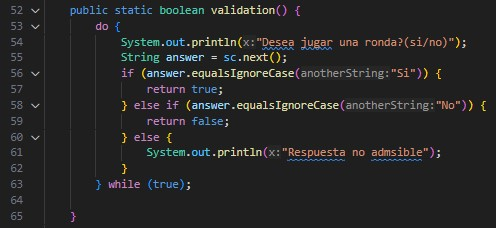
\includegraphics[width=1\textwidth,keepaspectratio]{img/validation.jpg}
		%\includesvg{img/automata.svg}
		%\label{img:mot2}
		%\caption{Product backlog.}
	\end{figure}	
	
	\begin{itemize}	
		\item Adicionalmente se implementa un método el cual se encargará de recepcionar si el usuario quiere seguir jugando. Este método es de laboratorios pasados.
	\end{itemize}
	
	\begin{lstlisting}[language=bash,caption={Commit: de043b03d19c52fc136cf3167d29a847991b6a47 }][H]
		git add Aplicacion.java
		git commit -m "Se crea la clase aplicacion que llama a todos las clases"			
		git push -u origin main
	\end{lstlisting}
	
	
	
	\begin{lstlisting}[language=bash,caption={Compilando y probando todo el juego }][H]
	Desea jugar una ronda?(si/no)
	si
	Elija su reino (Francia, Inglaterra, Moros, Roma, Castilla)
	Francia
	Elija su reino (Francia, Inglaterra, Moros, Roma, Castilla)
	Castilla
	[Archer: name=Archer4x8, row=4, column=8, attackLevel=7, defenseLevel=3, actualLife=3, speed=0, attitude=Repose, current=true, arrows=5]
	Swordsman: name=Swordsman6x1, row=6, column=1, attackLevel=10, defenseLevel=8, actualLife=8, speed=0, attitude=Repose, current=true, longSnow=1.0, shieldWalls=false]
	Spearman: name=Spearman7x1, row=7, column=1, attackLevel=5, defenseLevel=10, actualLife=6, speed=0, attitude=Repose, current=true, lonLance=1]
	Spearman: name=Spearman8x9, row=8, column=9, attackLevel=5, defenseLevel=10, actualLife=6, speed=0, attitude=Repose, current=true, lonLance=1]
	
	[Knight: name=Knight3x1, row=3, column=1, attackLevel=13, defenseLevel=7, actualLife=10, speed=0, attitude=Repose, current=true, currentWeapon=sword, horseRiding=false]
	Spearman: name=Spearman3x3, row=3, column=3, attackLevel=5, defenseLevel=10, actualLife=7, speed=0, attitude=Repose, current=true, lonLance=1]
	[Archer: name=Archer4x1, row=4, column=1, attackLevel=7, defenseLevel=3, actualLife=3, speed=0, attitude=Repose, current=true, arrows=5]
	Swordsman: name=Swordsman4x4, row=4, column=4, attackLevel=10, defenseLevel=8, actualLife=9, speed=0, attitude=Repose, current=true, longSnow=1.0, shieldWalls=false]
	Spearman: name=Spearman6x2, row=6, column=2, attackLevel=5, defenseLevel=10, actualLife=7, speed=0, attitude=Repose, current=true, lonLance=1]
	Swordsman: name=Swordsman9x6, row=9, column=6, attackLevel=10, defenseLevel=8, actualLife=9, speed=0, attitude=Repose, current=true, longSnow=1.0, shieldWalls=false]
	Spearman: name=Spearman9x10, row=9, column=10, attackLevel=5, defenseLevel=10, actualLife=6, speed=0, attitude=Repose, current=true, lonLance=1]
	Spearman: name=Spearman10x3, row=10, column=3, attackLevel=5, defenseLevel=10, actualLife=8, speed=0, attitude=Repose, current=true, lonLance=1]
	
	A        B           C          D            E           F             G            H           I             J 
	1|__________||__________||__________||__________||__________||__________||__________||__________||__________||__________|
	2|__________||__________||__________||__________||__________||__________||__________||__________||__________||__________|
	3|_C*Fr10*C_||__________||_C*Fl07*C_||__________||__________||__________||__________||__________||__________||__________|
	4|_C*Fa03*C_||__________||__________||_C*Fe09*C_||__________||__________||__________||_C*Ca03*C_||__________||__________|
	5|__________||__________||__________||__________||__________||__________||__________||__________||__________||__________|
	6|_C*Ce08*C_||_C*Fl07*C_||__________||__________||__________||__________||__________||__________||__________||__________|
	7|_C*Cl06*C_||__________||__________||__________||__________||__________||__________||__________||__________||__________|
	8|__________||__________||__________||__________||__________||__________||__________||__________||_C*Cl06*C_||__________|
	9|__________||__________||__________||__________||__________||_C*Fe09*C_||__________||__________||__________||_C*Fl06*C_|
	10|__________||__________||_C*Fl08*C_||__________||__________||__________||__________||__________||__________||__________|
	Contando los soldados
	Archer: 1 Knight: 0 Spearman: 2 Swordsman: 1 Total: 4 Ejercito 1:[I@41906a77
	Archer: 1 Knight: 1 Spearman: 4 Swordsman: 2 Total: 8 Ejercito 2:[I@4b9af9a9
	
	Datos de los soldados con mayor vida
	Swordsman: name=Swordsman6x1, row=6, column=1, attackLevel=10, defenseLevel=8, actualLife=8, speed=0, attitude=Repose, current=true, longSnow=1.0, shieldWalls=false]
	[Knight: name=Knight3x1, row=3, column=1, attackLevel=13, defenseLevel=7, actualLife=10, speed=0, attitude=Repose, current=true, currentWeapon=sword, horseRiding=false]
	
	Estadisticas de batalla:        Reino Francia: 28.048780487804876%      Reino Castilla: 71.95121951219512%      Salio como aleatorio: 97%
	Empate
	Desea jugar una ronda?(si/no)
	no
	\end{lstlisting}
	
	\begin{itemize}	
		\item Pido disculpas por la presentación del tablero y los datos de los soldados, ya son problemas de Latex y no tanto de mi código 
	\end{itemize}


	
	
	\subsection{Diagrama UML}
	
	\begin{figure}[H]
		\centering
		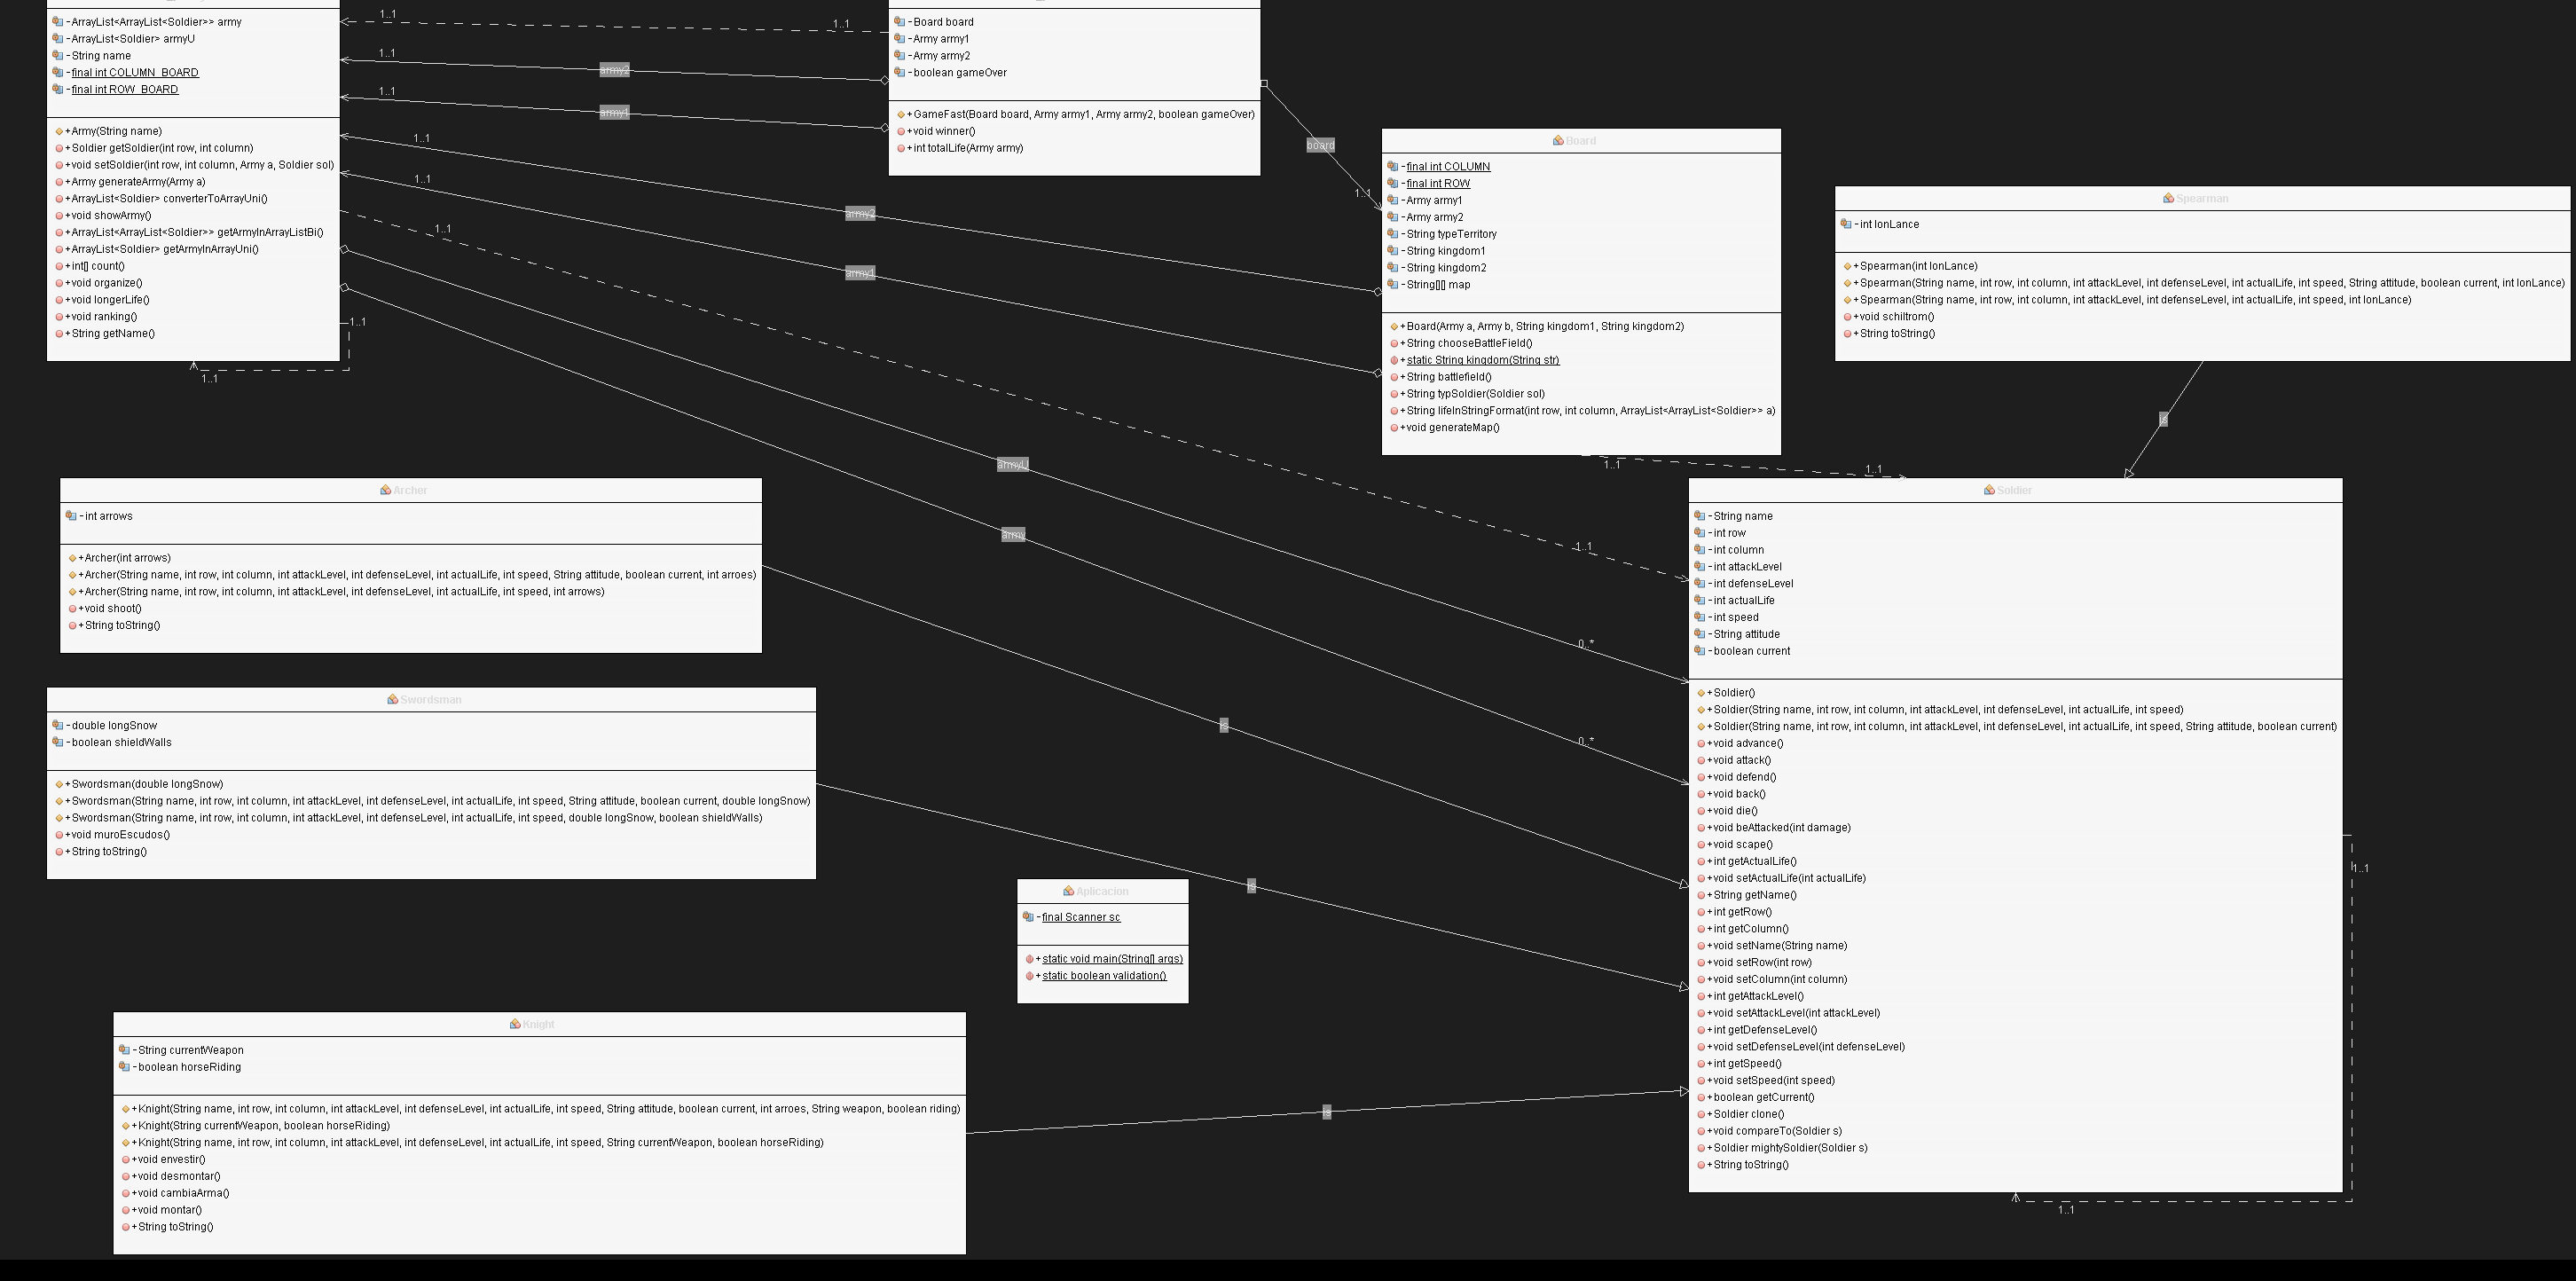
\includegraphics[width=1\textwidth,keepaspectratio]{img/uml.png}
		%\includesvg{img/automata.svg}
		%\label{img:mot2}
		%\caption{Product backlog.}
	\end{figure}
	
	\begin{itemize}	
			\item Si hay problemas en la visualización, puede ver la imagen en la carpeta img
	\end{itemize}
	
	\subsection{Estructura de laboratorio 20}
	\begin{itemize}	
		\item El contenido que se entrega en este laboratorio es el siguiente:
	\end{itemize}
	


	\begin{figure}[H]
		\centering
		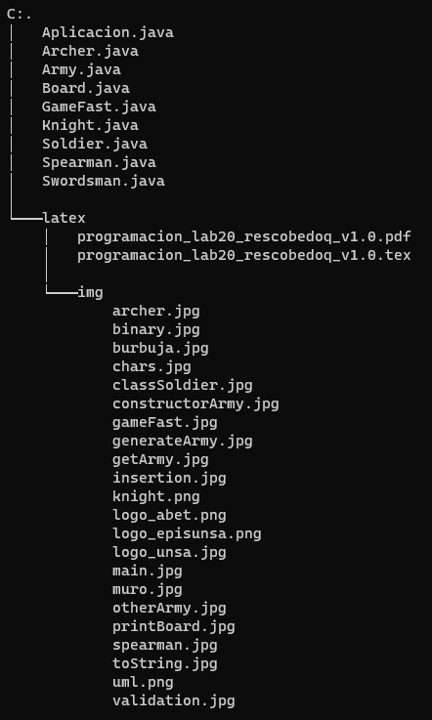
\includegraphics[width=0.8\textwidth,keepaspectratio]{img/tree.jpg}
		%\includesvg{img/automata.svg}
		%\label{img:mot2}
		%\caption{Product backlog.}
	\end{figure}	
	
	\begin{itemize}	
		\item Debido a problemas en la codificación de latex con ciertos caracteres que genera el comando tree f, se opta 
		por enviar la estructura de este laboratorio en formato de imagen
	\end{itemize}
	

   
	
	\section{\textcolor{red}{Rúbricas}}
	
	\subsection{\textcolor{red}{Entregable Informe}}
	\begin{table}[H]
		\caption{Tipo de Informe}
		\setlength{\tabcolsep}{0.5em} % for the horizontal padding
		{\renewcommand{\arraystretch}{1.5}% for the vertical padding
			\begin{tabular}{|p{3cm}|p{12cm}|}
				\hline
				\multicolumn{2}{|c|}{\textbf{\textcolor{red}{Informe}}}  \\
				\hline 
				\textbf{\textcolor{red}{Latex}} & \textcolor{blue}{El informe está en formato PDF desde Latex,  con un formato limpio (buena presentación) y facil de leer.}   \\ 
				\hline 
				
				
			\end{tabular}
		}
	\end{table}
	
	\clearpage
	
	\subsection{\textcolor{red}{Rúbrica para el contenido del Informe y demostración}}
	\begin{itemize}			
		\item El alumno debe marcar o dejar en blanco en celdas de la columna \textbf{Checklist} si cumplio con el ítem correspondiente.
		\item Si un alumno supera la fecha de entrega,  su calificación será sobre la nota mínima aprobada, siempre y cuando cumpla con todos lo items.
		\item El alumno debe autocalificarse en la columna \textbf{Estudiante} de acuerdo a la siguiente tabla:
		
		\begin{table}[ht]
			\caption{Niveles de desempeño}
			\begin{center}
				\begin{tabular}{ccccc}
					\hline
					& \multicolumn{4}{c}{Nivel}\\
					\cline{1-5}
					\textbf{Puntos} & Insatisfactorio 25\%& En Proceso 50\% & Satisfactorio 75\% & Sobresaliente 100\%\\
					\textbf{2.0}&0.5&1.0&1.5&2.0\\
					\textbf{4.0}&1.0&2.0&3.0&4.0\\
					\hline
				\end{tabular}
			\end{center}
		\end{table}	
		
	\end{itemize}
	
	\begin{table}[H]
		\caption{Rúbrica para contenido del Informe y demostración}
		\setlength{\tabcolsep}{0.5em} % for the horizontal padding
		{\renewcommand{\arraystretch}{1.5}% for the vertical padding
			%\begin{center}
			\begin{tabular}{|p{2.7cm}|p{7cm}|x{1.3cm}|p{1.2cm}|p{1.5cm}|p{1.1cm}|}
				\hline
				\multicolumn{2}{|c|}{Contenido y demostración} & Puntos & Checklist & Estudiante & Profesor\\
				\hline
				\textbf{1. GitHub} & Hay enlace URL activo del directorio para el  laboratorio hacia su repositorio GitHub con código fuente terminado y fácil de revisar. &2 &X &2 & \\ 
				\hline
				\textbf{2. Commits} &  Hay capturas de pantalla de los commits más importantes con sus explicaciones detalladas. (El profesor puede preguntar para refrendar calificación). &4 &X &4 & \\ 
				\hline 
				\textbf{3. Código fuente} &  Hay porciones de código fuente importantes con numeración y explicaciones detalladas de sus funciones. &2 &X &2 & \\ 
				\hline 
				\textbf{4. Ejecución} & Se incluyen ejecuciones/pruebas del código fuente  explicadas gradualmente. &2 &X &2 & \\ 
				\hline			
				\textbf{5. Pregunta} & Se responde con completitud a la pregunta formulada en la tarea.  (El profesor puede preguntar para refrendar calificación).  &2 &X &2 & \\ 
				\hline	
				\textbf{6. Fechas} & Las fechas de modificación del código fuente estan dentro de los plazos de fecha de entrega establecidos. &2 &X &2 & \\ 
				\hline 
				\textbf{7. Ortografía} & El documento no muestra errores ortográficos. &2 &X &2 & \\ 
				\hline 
				\textbf{8. Madurez} & El Informe muestra de manera general una evolución de la madurez del código fuente,  explicaciones puntuales pero precisas y un acabado impecable.   (El profesor puede preguntar para refrendar calificación).  &4 &X &2 & \\ 
				\hline
				\multicolumn{2}{|c|}{\textbf{Total}} &20 & &18 & \\ 
				\hline
			\end{tabular}
			%\end{center}
			%\label{tab:multicol}
		}
	\end{table}
	
	\clearpage
	
	\section{Referencias}
	\begin{itemize}			
		\item \url{https://www.geeksforgeeks.org/insertion-sort/}
	\end{itemize}	
	
	%\clearpage
	%\bibliographystyle{apalike}
	%\bibliographystyle{IEEEtranN}
	%\bibliography{bibliography}
	
\end{document}